\documentclass[tikz,border=10pt]{standalone}
\usetikzlibrary{calc}
\begin{document}
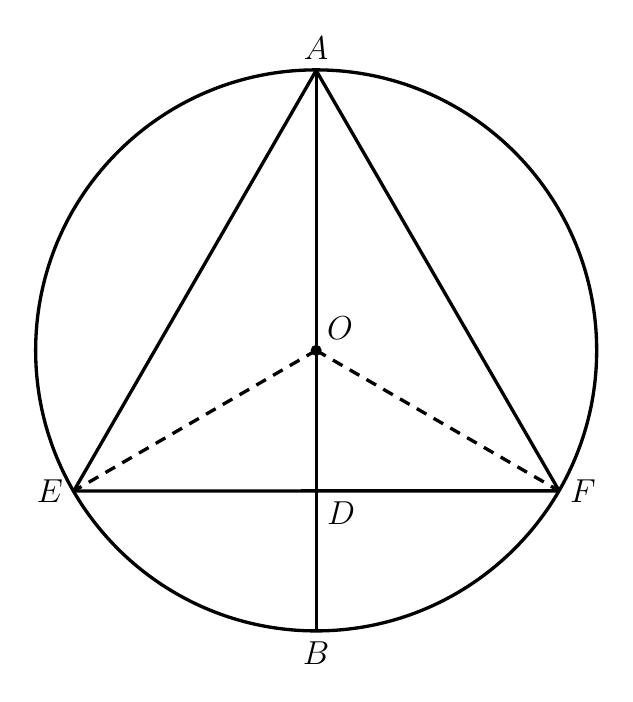
\begin{tikzpicture}[line join=round, line width=1.2pt]
% Coordinates in cm, origin at circle centre O
% scale s = 0.015094 cm/px, y flipped
\coordinate (O) at (0,0);
\coordinate (A) at (0,3.555);
\coordinate (B) at (0,-3.563);
\coordinate (E) at (-3.078,-1.785);
\coordinate (F) at (3.086,-1.784);
\coordinate (D) at (0,-1.785);

% Circle (radius 236 px)
\draw (O) circle[radius=3.5625];

% Solid chords and diameter
\draw (A) -- (B);
\draw (A) -- (E);
\draw (A) -- (F);
\draw (E) -- (F);

% Dashed radii
\draw[dash pattern=on 4pt off 3pt] (O) -- (E);
\draw[dash pattern=on 4pt off 3pt] (O) -- (F);

% Labels
\node[above, font=\fontsize{12}{14.4}\selectfont] at (A) {$A$};
\node[below, font=\fontsize{12}{14.4}\selectfont] at (B) {$B$};
\node[below right, font=\fontsize{12}{14.4}\selectfont] at (D) {$D$};
\node[left, font=\fontsize{12}{14.4}\selectfont] at (E) {$E$};
\node[right, font=\fontsize{12}{14.4}\selectfont] at (F) {$F$};
\node[above right, font=\fontsize{12}{14.4}\selectfont] at (O) {$O$};

% Centre dot at O (drawn last so it sits on top)
\fill (O) circle (2pt);
\end{tikzpicture}
\end{document}